\documentclass[letterpaper, 12pt]{article}

%%%%%%%%%%%%%%%%%%%%%%%%%%%%%
% DEFINITIONS
% Change those informations
% If you need umlauts you have to escape them, e.g. for an ü you have to write \"u
\gdef\mytitle{A04}
\gdef\mythema{Continuous Integration mit Jenkins}

\gdef\mysubject{Softwareentwicklung}
\gdef\mycourse{5BHIT 2017/18, GruppeA}
\gdef\myauthor{Nicolaus Rotter}

\gdef\myversion{0.2}
\gdef\mybegin{Begonnen am \today}
\gdef\myfinish{Beendet am \today}

\gdef\mygrade{Note:}
\gdef\myteacher{Betreuer: Dolezal}
%
%%%%%%%%%%%%%%%%%%%%%%%%%%%%%

%!TEX root=../document.tex

\usepackage[in]{fullpage}
% Fontencoding for possible copy&paste out of PDF
\usepackage[T1]{fontenc}
\usepackage[utf8]{inputenc}
\usepackage[ngerman]{babel}
\usepackage{graphicx} 
\usepackage{wasysym}
\usepackage{textcomp}
\usepackage{sectsty}
\usepackage{caption}
\usepackage{listings}
\usepackage{array}
\usepackage{colortbl}
\usepackage{footmisc}
\usepackage{fancyhdr}
\usepackage{ccicons}
\usepackage{suffix}
\usepackage{multirow}
\usepackage{tabularx}
\usepackage{listings}
\usepackage{accsupp}
\usepackage{color}
\usepackage{url}
\usepackage[dvipsnames]{xcolor}
\usepackage[longnamesfirst,nonamebreak]{natbib}
\usepackage[headsep=1cm,headheight=3cm,hmargin=2cm,vmargin=2.5cm]{geometry}
\usepackage[nolist]{acronym}

% Definitions for Textcolor
\usepackage{color}
\definecolor{listings}{rgb}{0.96, 0.96, 0.96}
\definecolor{update}{rgb}{1, 0.8, 0.8}
\definecolor{config}{rgb}{0.8, 1, 0.8}
\definecolor{gray}{rgb}{0.4,0.4,0.4}
\definecolor{darkblue}{rgb}{0.0,0.0,0.6}
\definecolor{cyan}{rgb}{0.0,0.6,0.6}

% Java Syntaxhighligthning
% strings
\definecolor{javared}{rgb}{0.6,0,0}
% comments
\definecolor{javagreen}{rgb}{0.25,0.5,0.35}
% keywords
\definecolor{javapurple}{rgb}{0.5,0,0.35}
% javadoc
\definecolor{javadocblue}{rgb}{0.25,0.35,0.75}

\lstset{
	basicstyle=\ttfamily\small,
	keywordstyle=\bfseries\color[rgb]{0.496,0.000,0.332},
	commentstyle=\color[rgb]{0.246,0.496,0.371},
	stringstyle=\color[rgb]{0.164,0.000,0.996},
	tabsize=4,
	breaklines=true,
	numbers=left,
	numberstyle=\tiny\color{black},
	stepnumber=2,
	numbersep=8pt,
	numberstyle=\tiny,
	captionpos=b,
	xleftmargin=1cm,
	showspaces=false,
	showstringspaces=false,
	basewidth={0.53em,0.45em},
	frame=single,
	xleftmargin=1cm,
	basicstyle=\scriptsize,
}


\lstdefinestyle{Java}{
	language=Java,
	keywordstyle=\color{javapurple}\bfseries,
	stringstyle=\color{javared},
	commentstyle=\color{javagreen},
	morecomment=[s][\color{javadocblue}]{/**}{*/},
}

\lstdefinelanguage{XML}
{
	morestring=[b]",
	morestring=[s]{>}{<},
	morecomment=[s]{<?}{?>},
	stringstyle=\color{black},
	identifierstyle=\color{darkblue},
	keywordstyle=\color{cyan},
	% list your attributes here
	morekeywords={xmlns,version,type}
}

\lstdefinestyle{XML}{
	language=XML,
	basicstyle=\ttfamily\small,
	columns=fullflexible,
	commentstyle=\color{gray}\upshape
}

\newcommand{\noncopynumber}[1]{
	\BeginAccSupp{method=escape,ActualText={}}
	#1
	\EndAccSupp{}
}
\lstdefinestyle{bash}{
	language=bash,
	basicstyle=\ttfamily\small,
	literate={-}{{-}}{1},
	% http://tex.stackexchange.com/questions/145416/how-to-have-straight-single-quotes-in-lstlistings
	upquote=true;
	showstringspaces=false,
	%numbers=none,
	% http://tex.stackexchange.com/questions/122256/only-select-code-without-line-numbers
	numberstyle=\tiny\noncopynumber,
	breaklines=false,
	columns=fullflexible,
	basicstyle=\scriptsize
}

% http://tex.stackexchange.com/questions/83085/how-to-improve-listings-display-of-json-files
\colorlet{punct}{red!60!black}
\definecolor{background}{HTML}{EEEEEE}
\definecolor{delim}{RGB}{20,105,176}
\colorlet{numb}{magenta!60!black}
\lstdefinelanguage{json}{
	basicstyle=\ttfamily\small,
	numbers=left,
	numberstyle=\scriptsize,
	stepnumber=2,
	numbersep=8pt,
	showstringspaces=false,
	breaklines=true,
	literate=
	*{0}{{{\color{numb}0}}}{1}
	{1}{{{\color{numb}1}}}{1}
	{2}{{{\color{numb}2}}}{1}
	{3}{{{\color{numb}3}}}{1}
	{4}{{{\color{numb}4}}}{1}
	{5}{{{\color{numb}5}}}{1}
	{6}{{{\color{numb}6}}}{1}
	{7}{{{\color{numb}7}}}{1}
	{8}{{{\color{numb}8}}}{1}
	{9}{{{\color{numb}9}}}{1}
	{:}{{{\color{punct}{:}}}}{1}
	{,}{{{\color{punct}{,}}}}{1}
	{\{}{{{\color{delim}{\{}}}}{1}
	{\}}{{{\color{delim}{\}}}}}{1}
	{[}{{{\color{delim}{[}}}}{1}
	{]}{{{\color{delim}{]}}}}{1},
	basicstyle=\scriptsize
}

\usepackage[
	colorlinks,
	citecolor=black,
	filecolor=black,
	linkcolor=black,
	urlcolor=black,
	linktoc=all
]{hyperref}


\let\tempsection\section
\renewcommand\section[1]{\vspace{-0.3cm}\tempsection{#1}\vspace{-0.3cm}}
\WithSuffix\newcommand\section*[1]{\tempsection*{#1}}

\let\tempsubsection\subsection
\renewcommand\subsection[1]{\vspace{0cm}\tempsubsection{#1}\vspace{0cm}}

\let\tempsubsubsection\subsubsection
\renewcommand\subsubsection[1]{\vspace{0cm}\tempsubsubsection{#1}\vspace{0cm}}

\linespread{0.94}

\lhead{\mysubject}
\chead{}
\rhead{\bfseries\mythema}
\lfoot{\mycourse}
\cfoot{\thepage}
% Creative Commons license BY
% http://creativecommons.org/licenses/?lang=de
\rfoot{\ccby\hspace{2mm}\myauthor}
\renewcommand{\headrulewidth}{0.4pt}
\renewcommand{\footrulewidth}{0.4pt}

\begin{document}
\parindent 0pt
\parskip 6pt

\pagenumbering{Roman} 
%!TEX root=../laborprotokoll.tex

\begin{titlepage}

	\begin{figure}[!h]
		\begin{flushright}
			
\includegraphics[width=0.3\linewidth]{images/jdIT_tgm.png}
		\end{flushright}
	\end{figure}

	\vspace{2.5cm} 

	{\begin{center} \bfseries\huge
			\rule{17.5cm}{0.1mm}  
			\\[5mm]
			\mytitle\\[5mm]
			\mythema\\
			\rule{17.5cm}{0.1mm}  
	\end{center}}

	{\begin{flushright} \bfseries\Large
			\vspace{2cm}
			\mysubject\\
			\mycourse\\[10mm]
			\myauthor\\[10mm]
	\end{flushright}}

	{\begin{table}[!h] \bfseries\normalsize
		\begin{tabularx}{\textwidth}{lXr @{\hspace{0mm}}}
			&& Version \myversion\\
			\mygrade && \mybegin\\
			\myteacher && \myfinish\\
		\end{tabularx}
	\end{table}}

\end{titlepage}


\clearpage
\thispagestyle{empty}
\tableofcontents

\newpage
\pagenumbering{arabic}
\pagestyle{fancy}

%\vspace{-0.5cm}

%!TEX root=../document.tex

\section{Einführung}
Lass das Bruch-Projekt mithilfe von Jenkins automatisch bei jedem Build testen!

\subsection{Aufgabenstellung}
Grundanforderungen:

\begin{itemize}
	\item Installiere auf deinem Rechner bzw. einer virtuellen Instanz das Continuous Integration System Jenkins
	\item Installiere die notwendigen Plugins für Jenkins (Violations, Cobertura)
	\item Installiere Nose, Coverage und Pylint (mithilfe von pip)
	\item Integriere dein Bruch-Projekt in Jenkins, indem du es mit Git verbindest
	\item Überlege dir und argumentiere eine sinnvolle Pull-Strategie
	\item Konfiguriere Jenkins so, dass deine Unit Tests automatisch bei jedem Build durchgeführt werden inkl. Berichte über erfolgreiche / fehlgeschlagene Tests und Coverage
	\item Protokolliere deine Vorgehensweise (inkl. Zeitaufwand, Konfiguration, Probleme) und die Ergebnisse (viele Screenshots!)
\end{itemize}

Erweiterungen:

\begin{itemize}
	\item Konfiguriere und teste eine Git-Hook, sodass Änderungen auf GitHub automatisch einen Build auslösen! Dokumentiere deine Vorgangsweise (mit Screenshots)!
	\item Recherchiere, wie mithilfe von Jenkins GUI-Tests durchgeführt werden können und baue selbstständig einen Beispiel-GUI-Test ein! Dokumentiere deine Vorgangsweise (mit Screenshots)!
	\item Lass deine Sphinx-Dokumentation automatisch mitbuilden und veröffentlichen! Dokumentiere deine Vorgangsweise (mit Screenshots)!
\end{itemize}


\clearpage

%!TEX root=../document.tex

\section{Grundanforderungen}
\label{sec:Ergebnisse}

\subsection{Installation Jenkins}

Der erste Punkt verlangt nach der Installation von Jenkins. Dafür wird die Software über die im Kurs abgelegte Verlinkung zu \textbf{https://jenkins.io/index.html} heruntergeladen. Nach der erfolgreichen installation sollte es möglich sein über den Browser auf \textbf{localhost:8080} Zugriff zu Jenkins zu bekommen. 

zunächst wurde ein neuer Benutzer mit Administrator-Rechten hinzugefügt. 
Dieser kann dann im /user/ - Tab eingesehen werden. 

\begin{figure}[!h]
	\begin{center}
		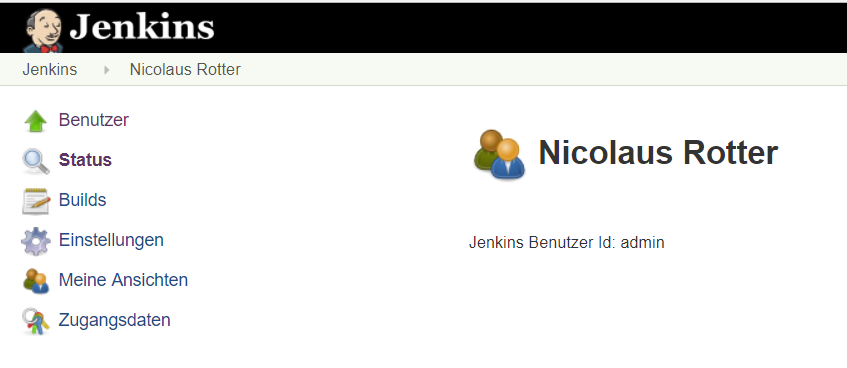
\includegraphics[width=0.7\textwidth]{images/userPNG.PNG}
	\end{center}
\end{figure}

\subsection{Installation Violations, Corbertura}

Zunächst wird die Installation der von uns benötigten Jenkins PlugIns verlangt. Dazu muss man auf \textbf{Jenkins verwalten -> PulgIns verwalten} gehen und im \textbf{Verfügbar}-Tab diese installieren. 

Falls dieser Schritt erfolgreich war sollten die PuligIns nach dem Neustart von Jenkins im \textbf{Installiert}-Tab erscheinen.

\subsection{Installation Nose, Coverage, Pylint}

Nun müssen folgende Packages über pip installiert werden:
\begin{itemize}
	\item Nose
	\item Coverage
	\item Pylint
\end{itemize}

\clearpage

Dies wurde im meinem Fall schon gemacht, daher bekomme ich folgende Rückmeldung in der Konsole:

\begin{figure}[!h]
	\begin{center}
		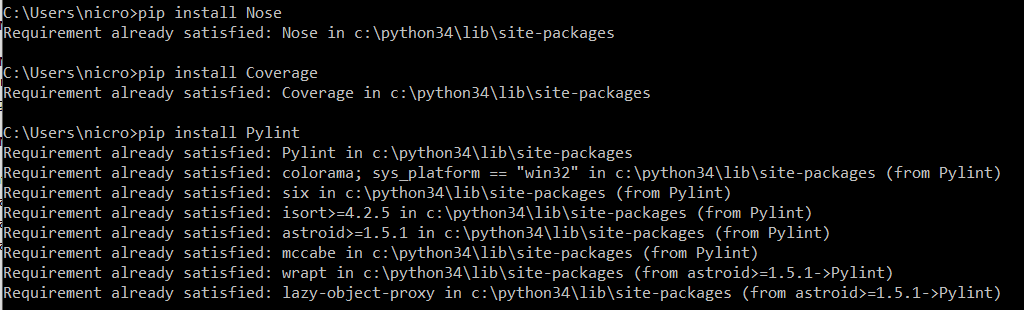
\includegraphics[width=0.7\textwidth]{images/pip.PNG}
	\end{center}
\end{figure}



\clearpage

\bibliographystyle{unsrt}
\bibliography{references}
\listoftables
\lstlistoflistings
\listoffigures

\end{document}
